\documentclass{beamer}
\usepackage{geometry}
\usepackage[english]{babel}
\usepackage[utf8]{inputenc}
\usepackage{amsmath}
\usepackage{amsfonts}
\usepackage{amssymb}
\usepackage{tikz}
\usetikzlibrary{quotes, angles}
\usepackage{graphicx}

\usepackage{multicol}
%\usepackage{pgfplots}
%\pgfplotsset{width=10cm,compat=1.9}
%\usepackage{pgfplotstable}

\usepackage{fancyhdr}
\pagestyle{fancy}
\setlength{\headheight}{12pt}%doesn't seem to fix warning
\fancyhf{}

%\rhead{\small{24 February 2020}}
\lhead{\small{BECA / Dr. Huson / Unit 11: Algebra competencies}}

\renewcommand{\headrulewidth}{0pt}

\title{Mathematics Class Slides}
\subtitle{Bronx Early College Academy}
\author{Chris Huson}
\date{21 April 2020}

\begin{document}
\frame{\titlepage}
\section[Outline]{}
\frame{\tableofcontents}

\section{11.0 Scanning and uploading written work to Gradescope, Wednesday 22 April} 
\frame
{
  \frametitle{GQ: How do we document our mathematical reasoning?}
  \framesubtitle{HSA.CED.A.4 Rearrange formulas to highlight a quantity of interest \hfill \alert{11.1 Wed. 22 April}}

  Written work must be submitted following standard protocols
  
  \begin{enumerate}
      \item Title and label (lined paper) \\[0.25cm]
      10.2 Geometry \hfill First, Last name \\
      11.1 Literals (\emph{Assignment})\\
      22 April 2020 (\emph{Date}) \\[0.25cm]
      Number problems down the left (drawings, notes on the right)
      \item Photograph and convert to pdf with an app: \\
      \quad Adobe Scan, Evernote Scannable, or Genius Scan
      \item Login and upload to Gradescope.com (class code: \alert{MG8X2G})
    \end{enumerate}
}

\section{11.1 Algebra review, Literals, Wednesday 22 April} 
\frame
{
  \frametitle{GQ: How do we apply algebra to equations with literals?}
  \framesubtitle{HSA.CED.A.4 Rearrange formulas to highlight a quantity of interest \hfill \alert{11.1 Wed. 22 April}}

  \begin{block}{Do Now: Submit Present; Answer these questions by chat}
    \begin{itemize}
      \item What's the best day for Chess Club? \\
      (Congratulations chess champion Ahmed!)
      \item What type of phone do you have? 
    \end{itemize}

    \end{block}
    Tech: turning in written work by uploading to Gradescope \\[0.25cm]
    Lesson: \\
    Solving equations with multiple unknowns\\
    Deltamath practice problems \\[0.25cm]
    Homework: Complete handout problem set, due by 10:00pm \\
    (submit on time for full credit. late work: 80\%)
}

\frame
{
  \frametitle{GQ: How do we apply algebra to equations with literals?}
  \framesubtitle{HSA.CED.A.4 Rearrange formulas to highlight a quantity of interest \hfill \alert{11.1 Wed. 22 April}}

  \Large{
  Simplify each expression by ``collecting like terms''
  
  \begin{enumerate}
    \begin{multicols}{2}
      \item $3x+2x$ \vspace{2cm}
      \item $5\pi-2\pi+4\pi$
    \end{multicols}
    \end{enumerate} \vspace{5cm}
}
}


\frame
{
  \frametitle{GQ: How do we apply algebra to equations with literals?}
  \framesubtitle{HSA.CED.A.4 Rearrange formulas to highlight a quantity of interest \hfill \alert{11.1 Wed. 22 April}}

  
  Simplify each expression by ``collecting like terms''
  
  \begin{enumerate}
    \begin{multicols}{2}
      \item $3x+2x$
      \begin{itemize}
        \item[$\square$] $5+x$
        \item[$\square$] $(x+x+x)+(x+x)$
        \item[$\square$] $5x$
        \item[$\square$] $(3+2)x$
      \end{itemize}
      \item $5\pi-2\pi+4\pi$
      \begin{itemize}
        \item[$\square$] $3\pi+4$
        \item[$\square$] $(5-2+4)\pi$
        \item[$\square$] $7+\pi$
        \item[$\square$] $7 \times \pi$
      \end{itemize}
    \end{multicols}
    \end{enumerate} \vspace{5cm}
}

\frame
{
  \frametitle{GQ: How do we apply algebra to equations with literals?}
  \framesubtitle{HSA.CED.A.4 Rearrange formulas to highlight a quantity of interest \hfill \alert{11.1 Wed. 22 April}}

  Simplify each expression by ``collecting like terms''
\Large{  
  \begin{enumerate}%[itemsep=2cm]
    \begin{multicols}{2}
      \item $3x-2x+7y$ \vspace{2cm}
      \item $5z+5\pi-2\pi+z$
      \item $-k+7\sqrt{2}+2k+3\sqrt{2}$ \vspace{2cm}
      \item $5\pi x-2 \pi x +9y$
    \end{multicols}
    \end{enumerate} \vspace{2cm}
}}


\frame
{
  \frametitle{GQ: How do we apply algebra to equations with literals?}
  \framesubtitle{HSA.CED.A.4 Rearrange formulas to highlight a quantity of interest \hfill \alert{11.1 Wed. 22 April}}
  \Large{
  Solve each equation for the unknown
  
  \begin{enumerate}
    \begin{multicols}{2}
      \item $\displaystyle \frac{k}{\sqrt{3}}=11$
      \item $5z-2 \pi = 4\pi +z$
    \end{multicols}
    \end{enumerate} \vspace{7cm}
}}

\frame
{
  \frametitle{GQ: How do we apply algebra to equations with literals?}
  \framesubtitle{HSA.CED.A.4 Rearrange formulas to highlight a quantity of interest \hfill \alert{11.1 Wed. 22 April}}
  \Large{
  Solve each equation for the unknown
  
  \begin{enumerate}%[itemsep=2cm]
    \begin{multicols}{2}
      \item $4x-x\sqrt{3}=11$
      \item $5\pi x-2 \pi x= \pi x +14$
    \end{multicols}
    \end{enumerate} \vspace{7cm}
}}

\section{11.2 Literals, radicals, trig conventions Friday 24 April} 
\frame
{
  \frametitle{GQ: How do we apply algebra to equations with literals?}
  \framesubtitle{HSA.CED.A.4 Rearrange formulas to highlight a quantity of interest \hfill \alert{11.2 Friday 24 April}}

  \begin{block}{Do Now: Submit Present; Answer the question by chat}
    \begin{itemize}
      \item Give an example of a \emph{literal}, a value expressed with a symbol (do not use $x$)
    \end{itemize}

    \end{block}
    Chess Club tournament today 1:30 - 2:30 (\href{http://LiChess.org}{LiChess}) \\[0.25cm]
    Lesson: Operations on radicals (square roots)\\
    Applications with literals from trigonometry, science\\[0.25cm]
    Deltamath practice problems \\[0.25cm]
    Homework: Complete handout problem set, due by 10:00pm}

\frame
{
  \frametitle{Properties of square roots}

  \Large{
  Definition: $(\sqrt{a})^2=a$ \hfill note: $(-\sqrt{a})^2=a$ \\[1cm]

  Addition \\
  $\sqrt{b}+\sqrt{b}=2\sqrt{b}$, \hfill but $\sqrt{a}+\sqrt{b}=\sqrt{a}+\sqrt{b}$ \\[1cm]
  Multiplication \hfill  Inverse (reciprocal)\\
  $\sqrt{c} \times \sqrt{d}=\sqrt{cd}$ \hfill 
  $\displaystyle \sqrt{\frac{1}{k}}= \frac{1}{\sqrt{k}}$\\[0.5cm]
  
}
}

\frame
{
  \frametitle{Notation conventions}

  \Large{
  Greek letters: \\[0.25cm]
  $\alpha$ alpha, $\beta$ beta, $\gamma$ gamma, $\delta$ delta, $\epsilon$ epsilon\\[0.25cm]
  $\pi$ pi, $\theta$ theta, $\sigma$ sigma, $\phi$ phi \\[0.25cm]
  Capital Greek letters: $\Sigma$ Sigma, $\Delta$ Delta\\[1cm]
  Angle measures: 
  $45^\circ$, $\displaystyle \frac{5}{6}\pi$ radians, $x$, $\theta$, $A$

}
}

\frame
{
  \frametitle{Trigonometry situations}
  \framesubtitle{The tangent of an angle in a right triangle is the ratio of the opposite side's length to the length of the leg adjacent to the angle}

  \Large{
Solve for the missing side length, $x$
  \begin{enumerate}
    \begin{multicols}{2}
      \item $\displaystyle \tan \theta=\frac{x}{10}$
      \item $\displaystyle \tan \theta=\frac{20}{x}$
    \end{multicols}
    \end{enumerate} \vspace{5cm}
}
}

\section{11.3 Literals, radicals, trig conventions Wednesday 29 April} 
\frame
{
  \frametitle{GQ: How do we simplify radicals?}
  \framesubtitle{HSA.CED.A.4 Rearrange formulas to highlight a quantity of interest \hfill \alert{11.3 Wed. 29 April}}

  \begin{block}{Do Now: Submit Present; Answer the Google form}
    \begin{itemize}
      \item Solve for $x$: $4x-15y-z= 20+y-5z$
      \item Solve for $k$: $3k-mk+7=np$
    \end{itemize}
    \end{block}
    Review: literals in equations\\[0.25cm]
    Lesson: Simplifying radicals (square roots) by factoring\\
    Deltamath practice problems \\[0.25cm]
    Homework: Complete handout problem set, due by 10:00pm}


\section{11.3 Literals, radicals, trig conventions Thursday 30 April} 
\frame
{
  \frametitle{GQ: How do we simplify radicals?}
  \framesubtitle{HSA.CED.A.4 Rearrange formulas to highlight a quantity of interest \hfill \alert{11.3 Thurs 30 April}}

  \begin{block}{Do Now: Submit Present; Answer the Google form} \vspace{0.5cm}
    Solve for $x$: $4x-15y-z= 20+y-5z$
    \begin{multicols}{2}
    \begin{enumerate}[(a)]
      \item $x= 16y-4z+20$
      \item $x= 4y+z-5$
      \item $x= 4y-z+5$
      \item $x= 4y-4z+20$
    \end{enumerate}
  \end{multicols}
    \end{block}
    Review: literals in equations (e.g. $V=\frac{1}{3}\pi r^2h$, solve for $r$)\\[0.25cm]
    Lesson: Simplifying radicals (square roots) by factoring\\
    Deltamath practice problems \\[0.25cm]
    Homework: Complete handout problem set, due by 10:00pm}

\section{11.4 Cosine and sine Monday 4 May} 
\frame
{
  \frametitle{GQ: How do we use cosine and sine ratios?}
  \framesubtitle{HSA.CED.A.4 Rearrange formulas to highlight a quantity of interest \hfill \alert{11.4 Monday 4 May}}

  \begin{block}{Do Now: Submit Present; Answer the Google form} \vspace{0.5cm}
    \begin{multicols}{2}
      $\triangle ABC$ in standard position: vertex $A$ at $(0,0)$, right $\angle C$ above $x$-axis
      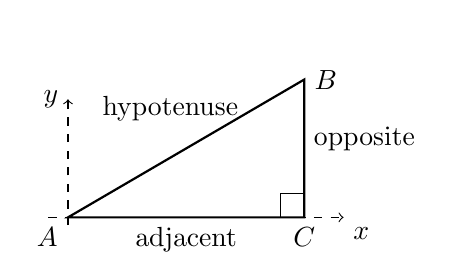
\begin{tikzpicture}[scale=0.5]
        \draw [dashed, ->] (-0.5,0) -- (7,0) node [below right] {$x$};
        \draw [dashed, ->] (0,-0.2)--(0,3) node [left] {$y$};
        \draw [thick]
        (0,0)node[below left]{$A$}--
        (6,0)node[below]{$C$}--
        (6,3.5)node[right]{$B$}--cycle;
        \draw (6,0)++(-0.6,0)--++(0,0.6)--+(0.6,0);
        \node at (3,0)[below]{adjacent};
        \node at (6,2)[right]{opposite};
        \node at (2.6,2.2)[above]{hypotenuse};
      \end{tikzpicture}
  \end{multicols}
    \end{block}
    Review: Pythagorean theorem; tangent (opposite over adjacent)\\[0.25cm]
    Lesson: Cosine and sine ratios, 
    Deltamath practice problems \\[0.25cm]
    Homework: Complete handout problem set, due by 10:00pm}

\section{11.4 Cosine and sine (10.3) Wednesday 6 May} 
\frame
{
  \frametitle{GQ: How do we use cosine and sine ratios?}
  \framesubtitle{HSA.CED.A.4 Rearrange formulas to highlight a quantity of interest \hfill \alert{11.4 Wednesday 6 May}}

  \begin{block}{Do Now: Submit Present; Answer the Google form} \vspace{0.5cm}
    \begin{multicols}{2}
      $\triangle ABC$ in standard position: vertex $A$ at $(0,0)$, right $\angle C$ above $x$-axis
      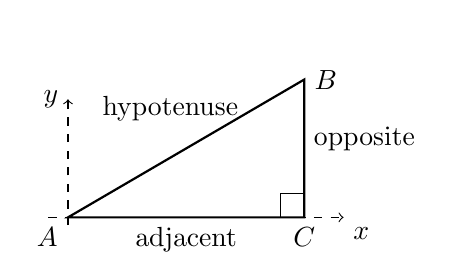
\begin{tikzpicture}[scale=0.5]
        \draw [dashed, ->] (-0.5,0) -- (7,0) node [below right] {$x$};
        \draw [dashed, ->] (0,-0.2)--(0,3) node [left] {$y$};
        \draw [thick]
        (0,0)node[below left]{$A$}--
        (6,0)node[below]{$C$}--
        (6,3.5)node[right]{$B$}--cycle;
        \draw (6,0)++(-0.6,0)--++(0,0.6)--+(0.6,0);
        \node at (3,0)[below]{adjacent};
        \node at (6,2)[right]{opposite};
        \node at (2.6,2.2)[above]{hypotenuse};
      \end{tikzpicture}
  \end{multicols}
    \end{block}
    Review: Pythagorean theorem; tangent (opposite over adjacent)\\[0.25cm]
    Lesson: Cosine and sine ratios, 
    Peardeck group work problem set}

\end{document}

Given right triangle PQR with right angle R. If PR=4, QR=3, PQ=5. 
Find the tangent of angle P as a ratio.

